\section{Analysis of architectures}
\begin{minipage}{0.4\linewidth}
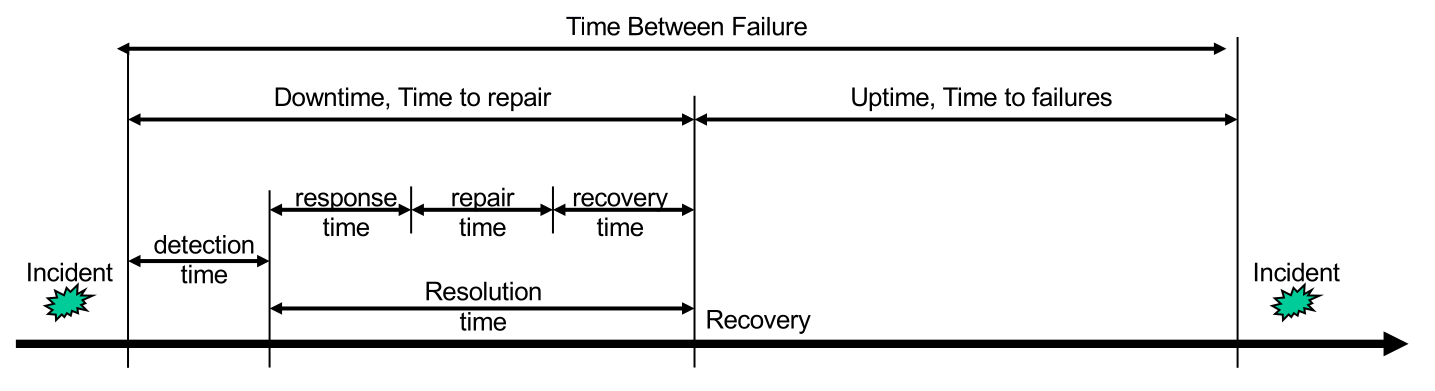
\includegraphics[angle=90, origin=c, width=\linewidth]{6-design/lifecycle-failure.png}
\end{minipage}
\begin{minipage}{0.58\linewidth}
\textbf{Time of occurence}: time at which the user becomes aware of the fault.\\
\textbf{Detection time}: the service provider is informed.\\
\textbf{Response time}: time required by the service provider to respond to the user.\\
\textbf{Repair time}: time required to restore the service or the component that caused the fault.\\
\textbf{Recovery time}: time required to restore the system.\\ \\
\textbf{Mean Time To Repair (MTTR)}: average time between the occurrence of a fault and recovery.\\
\textbf{Mean Time To Failures (MTTF)}: average time between the recovery of an incident and the occurence of the next one.\\
\textbf{Mean Time Between Failures (MTBF)}: average time between the occurrence of two consecutive faults.\\ \\

$MTBF = MTTR + MTTF$.
\end{minipage}

\subsection{Availability}
Probability that a component is working properly at a given time.
\[ A = \frac{MTTF}{MTTF + MTTR} \]

Availability in series: $A = \prod A_i$\\
Availability in parallel: $A = 1 - \prod (1 - A_i)$

\subsection{Reliability}
Probability that a component has always been working properly during a time interval $(0, t)$.
\[ R = e^{-\lambda t} \qquad \lambda =\frac{1}{MTTF} \]